\documentclass[a4paper]{article}

\usepackage[english]{babel}
\usepackage[utf8]{inputenc}
\usepackage{amsmath}
\usepackage{graphicx}
\usepackage[colorinlistoftodos]{todonotes}
% 导入包
\usepackage{hyperref}
% 格式设置
\hypersetup{hidelinks,
	colorlinks=true,
	allcolors=black,
	pdfstartview=Fit,
	breaklinks=true}
	
\title{DAT094 Lab 2: Arithmetic and hierarchy}

\author{Weihan Gao – weihanga@chalmers.se}

\date{\today}

\begin{document}
\sloppy
\maketitle




\section{Communicating FSMs}
\label{sec:introduction}



In Lab1, the SPI was implemented by a big FSM, where we can find 4 states -- “A\_B”, “zero”, “GA”, and “SHDN” for header bits transit and 12 states for 12-bit data’s transit correspondingly. So it can be easily separated into two parts according to the type of data on the SDI. And we can also take apart the big FSM into two small FSMs to control what kind of data should be transmitted in order. Small doesn’t mean non-hierarchy. In my design, I create a main FSM named FSM2 and a sub-FSM named FSM1. Unlike the big FSM before, FSM2 only generates header bits instead of data bits. To generate the data bits, it has the power to wake sub-FSM up at any time. But only when the “SHDN\_state” in FSM2 is over is the proper time. 


\begin{figure}[h]
\centering
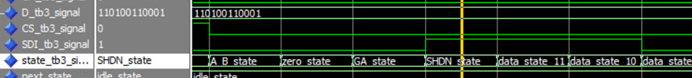
\includegraphics[width=1\textwidth]{fig9.png}
\caption{\label{fig:data}States in lab1}
\end{figure}


\begin{figure}[h]
\centering
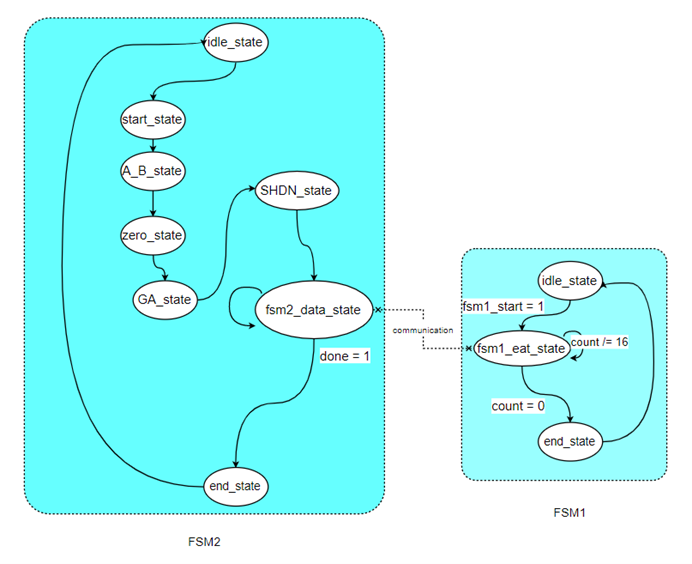
\includegraphics[width=9.5cm,height=8.5cm]{fig10.png}
\caption{\label{fig:data}FSMs}
\end{figure}

Splitting a big FSM into a main and sub-FSMs can distribute some assignments, such as addresses counting or waiting, to a sub-FSM even more. The main FSM focus on how to control them. But in some high-speed required cases, the communications between the main and sub FSMs will slow down the speed, I think.


Since the division of labor, signal communication is important between them. The “load” and “start” signals from FSM2 ask FSM1 to load data from the “din” port and to push the data bits one by one. FSM1 also needs the feedback -- “done” signal to tell the main FSM that data bits are over. I forgot to add data communication between main and sub in designing once (asking someone to help you withdraw money but forgetting to take money from him is TERRIBLE, FSM2 must agree), the data communication is completed finally by a single interconnect data wire. Importantly that data communication, instruction communication, and feedback communication are necessary.





\begin{figure}[h]
\centering
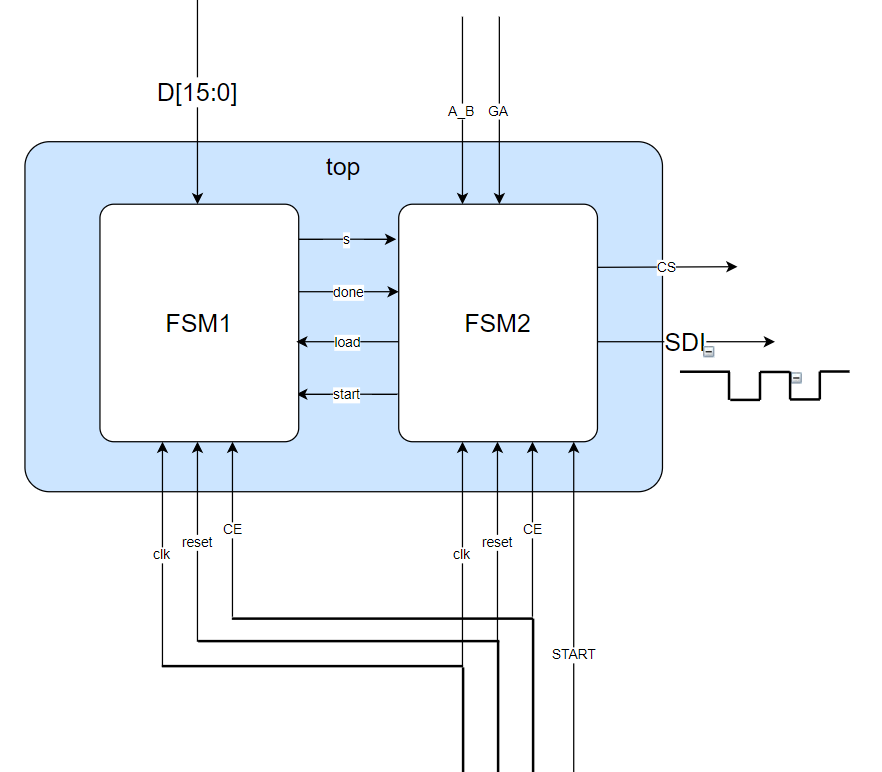
\includegraphics[width=1\textwidth]{fig11.png}
\caption{\label{fig:data}Block diagram of FSM 1, FSM 2, and the container}
\end{figure}

With 4 interconnect wires, we can assemble FSM1 and FSM2 together in the TOP file design (it is called the “container” in the document), whose behavior and port are equal to the SPI file in Lab1 almost. Sixteen-bit width data is set as an input signal of TOP and FSM1, One-bit width signal, named SDI, is an output of FSM2 and TOP. System clock, reset, and enable clock are input signals for the three. It is a little confusing that FSM1 needs the enable clock even if it is sub-FSM not the main. The low frequency “CE” can synchronize sub-FSM and main-FSM in fit. Moreover, if creating a counter in sub-FSM to wait for the data pushing, the counter is counting for “CE” rather than the system clock – “clk”. So the two FSMs need to connect to the “CE” both.










\end{document}